%%%%%%%%%%%%%%%%%%%%%%%%%%%%%%%%%%%%%%%%%
% Lachaise Assignment
% LaTeX Template
% Version 1.0 (26/6/2018)
%
% This template originates from:
% http://www.LaTeXTemplates.com
%
% Authors:
% Marion Lachaise & François Févotte
% Vel (vel@LaTeXTemplates.com)
%
% License:
% CC BY-NC-SA 3.0 (http://creativecommons.org/licenses/by-nc-sa/3.0/)
% 
%%%%%%%%%%%%%%%%%%%%%%%%%%%%%%%%%%%%%%%%%

%----------------------------------------------------------------------------------------
%	PACKAGES AND OTHER DOCUMENT CONFIGURATIONS
%----------------------------------------------------------------------------------------

\documentclass{article}
\usepackage{mathtools}
\usepackage{physics}
\usepackage{amsmath}
\input{structure.tex} % Include the file specifying the document structure and custom commands

%----------------------------------------------------------------------------------------
%	ASSIGNMENT INFORMATION
%----------------------------------------------------------------------------------------

\title{Quantum Computing Project} % Title of the assignment

\author{Tiernan\\ Riddhi\\ Jeb\\ Finn \\ Han \\ Yi Sheng}  % Author name and email address

\date{University of Edinburgh --- \today} % University, school and/or department name(s) and a date

%----------------------------------------------------------------------------------------

\begin{document}

\maketitle % Print the title

%----------------------------------------------------------------------------------------
%	INTRODUCTION
%----------------------------------------------------------------------------------------
\vspace{10mm}
\hrule

\vspace{10mm}

\section*{Introduction} % Unnumbered section
\vspace{10mm}

The objective of our project is to build an application which implements the Grover's Algorithm to perform an unstructured search from a list of information. 
\vspace{5mm}

The programming language used in our project is Python. We use Git to plan, manage and organise the codes and work flow of this project. 
\vspace{5mm}

The aim of this project is to demonstrate the basic working principle of Grover's Algorithm in a shape of a simple GUI with input and output feature.
\pagebreak

\tableofcontents % Unnumbered section
\pagebreak

\section{Grover's Algorithm}
\subsection{Introduction}

The Grover's Algorithm is a quantum search algorithm which increases quadratically the speed of unstructured search. It is uses  amplitude amplification to search an unstructured set of $N$ elements/items. 

\subsection{Unstructured Search}
\vspace{10mm}

\begin{center}



\tikzset{every picture/.style={line width=0.75pt}} %set default line width to 0.75pt        

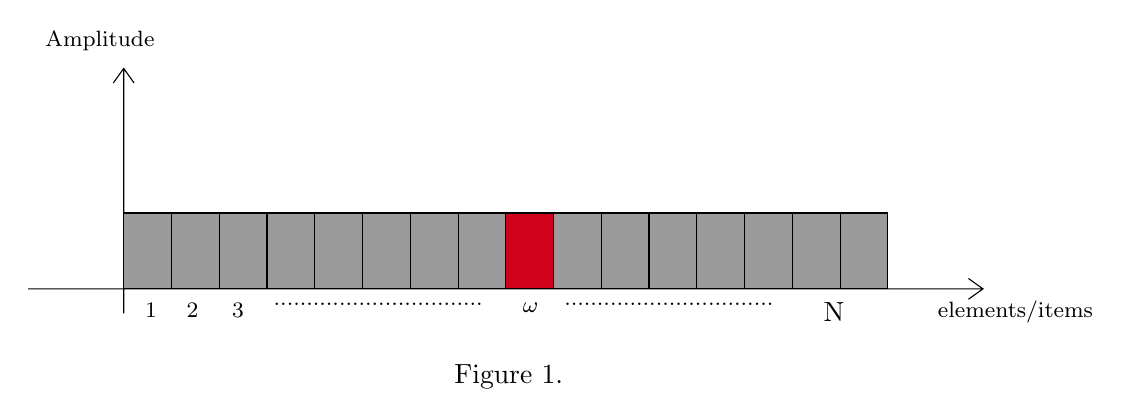
\begin{tikzpicture}[x=0.75pt,y=0.75pt,yscale=-1,xscale=1]
%uncomment if require: \path (0,310); %set diagram left start at 0, and has height of 310

%Shape: Axis 2D [id:dp7326811016330554] 
\draw  (54,256.57) -- (514,256.57)(100,150.37) -- (100,268.37) (507,251.57) -- (514,256.57) -- (507,261.57) (95,157.37) -- (100,150.37) -- (105,157.37)  ;
%Shape: Rectangle [id:dp9165080769461678] 
\draw  [fill={rgb, 255:red, 155; green, 155; blue, 155 }  ,fill opacity=1 ] (100,220) -- (123.02,220) -- (123.02,256.57) -- (100,256.57) -- cycle ;
%Shape: Rectangle [id:dp6197087457024866] 
\draw  [fill={rgb, 255:red, 155; green, 155; blue, 155 }  ,fill opacity=1 ] (123.02,220) -- (146.04,220) -- (146.04,256.57) -- (123.02,256.57) -- cycle ;
%Shape: Rectangle [id:dp5818508515663341] 
\draw  [fill={rgb, 255:red, 155; green, 155; blue, 155 }  ,fill opacity=1 ] (146.04,220) -- (169.06,220) -- (169.06,256.57) -- (146.04,256.57) -- cycle ;
%Shape: Rectangle [id:dp6466988498042014] 
\draw  [fill={rgb, 255:red, 155; green, 155; blue, 155 }  ,fill opacity=1 ] (169.06,220) -- (192.08,220) -- (192.08,256.57) -- (169.06,256.57) -- cycle ;
%Shape: Rectangle [id:dp9241747490680354] 
\draw  [fill={rgb, 255:red, 155; green, 155; blue, 155 }  ,fill opacity=1 ] (192.08,220) -- (215.1,220) -- (215.1,256.57) -- (192.08,256.57) -- cycle ;
%Shape: Rectangle [id:dp6900943731279547] 
\draw  [fill={rgb, 255:red, 155; green, 155; blue, 155 }  ,fill opacity=1 ] (215.1,220) -- (238.12,220) -- (238.12,256.57) -- (215.1,256.57) -- cycle ;
%Shape: Rectangle [id:dp9784662305616809] 
\draw  [fill={rgb, 255:red, 155; green, 155; blue, 155 }  ,fill opacity=1 ] (238.12,220) -- (261.14,220) -- (261.14,256.57) -- (238.12,256.57) -- cycle ;
%Shape: Rectangle [id:dp3189854749942387] 
\draw  [fill={rgb, 255:red, 155; green, 155; blue, 155 }  ,fill opacity=1 ] (261.14,220) -- (284.16,220) -- (284.16,256.57) -- (261.14,256.57) -- cycle ;
%Shape: Rectangle [id:dp19644432939638312] 
\draw  [fill={rgb, 255:red, 208; green, 2; blue, 27 }  ,fill opacity=1 ] (284.04,220) -- (307.06,220) -- (307.06,256.57) -- (284.04,256.57) -- cycle ;
%Shape: Rectangle [id:dp4454731461786199] 
\draw  [fill={rgb, 255:red, 155; green, 155; blue, 155 }  ,fill opacity=1 ] (307.06,220) -- (330.08,220) -- (330.08,256.57) -- (307.06,256.57) -- cycle ;
%Shape: Rectangle [id:dp8963311487850567] 
\draw  [fill={rgb, 255:red, 155; green, 155; blue, 155 }  ,fill opacity=1 ] (330.08,220) -- (353.1,220) -- (353.1,256.57) -- (330.08,256.57) -- cycle ;
%Shape: Rectangle [id:dp8621164913285171] 
\draw  [fill={rgb, 255:red, 155; green, 155; blue, 155 }  ,fill opacity=1 ] (353.1,220) -- (376.12,220) -- (376.12,256.57) -- (353.1,256.57) -- cycle ;
%Shape: Rectangle [id:dp7667099225825136] 
\draw  [fill={rgb, 255:red, 155; green, 155; blue, 155 }  ,fill opacity=1 ] (376.12,220) -- (399.14,220) -- (399.14,256.57) -- (376.12,256.57) -- cycle ;
%Shape: Rectangle [id:dp1405504024872024] 
\draw  [fill={rgb, 255:red, 155; green, 155; blue, 155 }  ,fill opacity=1 ] (399.14,220) -- (422.16,220) -- (422.16,256.57) -- (399.14,256.57) -- cycle ;
%Shape: Rectangle [id:dp6549374163542783] 
\draw  [fill={rgb, 255:red, 155; green, 155; blue, 155 }  ,fill opacity=1 ] (422.16,220) -- (445.18,220) -- (445.18,256.57) -- (422.16,256.57) -- cycle ;
%Shape: Rectangle [id:dp26369533307147797] 
\draw  [fill={rgb, 255:red, 155; green, 155; blue, 155 }  ,fill opacity=1 ] (445.18,220) -- (468.2,220) -- (468.2,256.57) -- (445.18,256.57) -- cycle ;

% Text Node
\draw (491,261) node [anchor=north west][inner sep=0.75pt]   [align=left] {{\footnotesize elements/items}};
% Text Node
\draw (61,131) node [anchor=north west][inner sep=0.75pt]   [align=left] {{\footnotesize Amplitude}};
% Text Node
\draw (109,262) node [anchor=north west][inner sep=0.75pt]  [font=\footnotesize] [align=left] {1};
% Text Node
\draw (129,262) node [anchor=north west][inner sep=0.75pt]  [font=\footnotesize] [align=left] {2};
% Text Node
\draw (171,262) node [anchor=north west][inner sep=0.75pt]  [font=\footnotesize] [align=left] {................................};
% Text Node
\draw (151,262) node [anchor=north west][inner sep=0.75pt]  [font=\footnotesize] [align=left] {3};
% Text Node
\draw (311,262) node [anchor=north west][inner sep=0.75pt]  [font=\footnotesize] [align=left] {................................};
% Text Node
\draw (291,262) node [anchor=north west][inner sep=0.75pt]  [font=\footnotesize] [align=left] {$\displaystyle \omega $};
% Text Node
\draw (436,262) node [anchor=north west][inner sep=0.75pt]   [align=left] {N};
% Text Node
\draw (258,292) node [anchor=north west][inner sep=0.75pt]   [align=left] {Figure 1.};


\end{tikzpicture}    
\end{center}
\vspace{10mm}
\noindent
An unstructured search through a list of items using Grover's Algorithm can be illustrated in Figure1. In this instance, $\omega$ the red block, represents the item which we want to find and $N$ represents the number of items in the list. 
\vspace{5mm}

\noindent
On classical computation, $\omega$ must check at least on average $O(N/2)$ entries of the list which gives $\frac{1}{2}$ the probability of finding $\omega$ or worse the entire N elements in the list.
With Grover's Algorithm, only $O(\sqrt{N})$ steps is required to find $\omega$.
\vspace{5mm}

\noindent
For an $N$ item search problem with $M$ number of solutions, the required number of times of searches will be $O(\sqrt{\frac{N}{M}})$.
\pagebreak

\subsection{The Oracle}
\vspace{10mm}

Let's suppose the function $f$ of $N$ integer such that $f:\{0,1, 2,...., N-1\} \rightarrow{\{0,1\}}$. The integers in the domain corresponds to the indices of the list and $f(x) =1$ if and only if $x$ corresponds to the item which is searched conversely $f(x) =0$ for $x$ not corresponding the item searched. There will be only one value of $x$ which satisfies $f(x)=1$ and this index corresponds to item $\omega$.
\noindent
\vspace{10mm}

So $f$ can be accessed with an unitary operator $U_{\omega}$ of  an oracle which satisfies:
\vspace{10mm}

$\hspace{30mm} \begin{cases}
      U_{\omega}\ket{x} = -\ket{x}  & \text{for} \ x = \omega, \ f(x) =1 \\
       U_{\omega}\ket{x} = \ket{x}  & \text{for} \ x \neq \omega, \ f(x) = 0 \\
\end{cases}$
\vspace{10mm}

The oracle function is defined as:
\vspace{10mm}

\qquad $\ket{x} \bigotimes\ \ket{q} \rightarrow{O_f} \ket{x} \bigotimes \ket{q \bigoplus f(x)}$ \footnote{$\bigotimes$ denotes tensor product and $\bigoplus$ denotes denotes addition modulo 2}
\vspace{5mm}

\qquad $\ket{q} = \frac{\ket{0} - \ket{1}}{\sqrt{2}}$
\vspace{5mm}

Substitute $\ket{q}$ into the oracle function $O_f$:
\vspace{5mm}

\qquad \qquad $ O\ket{x}\frac{\ket{0} - \ket{1}}{\sqrt{2}} \rightarrow \ket{x} \frac{\ket{f(x) \bigoplus 0} - \ket{f(x) \bigoplus 1}}{\sqrt{2}}$
\vspace{5mm}

\qquad if $ f(x) =1 \rightarrow \ket{x}\frac{\ket{f(x) \bigoplus0} - \ket{f(x) \bigoplus1}}{\sqrt{2}}$
\vspace{5mm}

\qquad if $f(x) =1 \rightarrow \ket{x}\frac{\ket{1 \bigoplus 0} - \ket{1 \bigoplus 1}}{\sqrt{2}} = -\ket{x}\frac{\ket{0} - \ket{1}}{\sqrt{2}}$
\vspace{5mm}

\qquad if $f(x) =0 \rightarrow \ket{x}\frac{\ket{0 \bigoplus 0} - \ket{0 \bigoplus 1}}{\sqrt{2}} = \ket{x}\frac{\ket{0} - \ket{1}}{\sqrt{2}}$
\vspace{5mm}

When $f(x) = 1 $, the amplitude $\ket{x}$ changed to negative and remains unchanged when $f(x) = 0$.

\section{Methodology}

\subsection{Workflow and Organization}

\subsection{Git}


\section{Coding with Python}


\subsection{Matrices}
\subsection{Gates}
\subsection{Tensor Products}

\section{Implementation}

Proin lobortis efficitur dictum. Pellentesque vitae pharetra eros, quis dignissim magna. Sed tellus leo, semper non vestibulum vel, tincidunt eu mi. Aenean pretium ut velit sed facilisis. Ut placerat urna facilisis dolor suscipit vehicula. Ut ut auctor nunc. Nulla non massa eros. Proin rhoncus arcu odio, eu lobortis metus sollicitudin eu. Duis maximus ex dui, id bibendum diam dignissim id. Aliquam quis lorem lorem. Phasellus sagittis aliquet dolor, vulputate cursus dolor convallis vel. Suspendisse eu tellus feugiat, bibendum lectus quis, fermentum nunc. Nunc euismod condimentum magna nec bibendum. Curabitur elementum nibh eu sem cursus, eu aliquam leo rutrum. Sed bibendum augue sit amet pharetra ullamcorper. Aenean congue sit amet tortor vitae feugiat.

In congue risus leo, in gravida enim viverra id. Donec eros mauris, bibendum vel dui at, tempor commodo augue. In vel lobortis lacus. Nam ornare ullamcorper mauris vel molestie. Maecenas vehicula ornare turpis, vitae fringilla orci consectetur vel. Nam pulvinar justo nec neque egestas tristique. Donec ac dolor at libero congue varius sed vitae lectus. Donec et tristique nulla, sit amet scelerisque orci. Maecenas a vestibulum lectus, vitae gravida nulla. Proin eget volutpat orci. Morbi eu aliquet turpis. Vivamus molestie urna quis tempor tristique. Proin hendrerit sem nec tempor sollicitudin.

% File contents
\begin{file}[hello.py]
\begin{lstlisting}[language=Python]
#! /usr/bin/python

import sys
sys.stdout.write("Hello World!\n")
\end{lstlisting}
\end{file}

Fusce eleifend porttitor arcu, id accumsan elit pharetra eget. Mauris luctus velit sit amet est sodales rhoncus. Donec cursus suscipit justo, sed tristique ipsum fermentum nec. Ut tortor ex, ullamcorper varius congue in, efficitur a tellus. Vivamus ut rutrum nisi. Phasellus sit amet enim efficitur, aliquam nulla id, lacinia mauris. Quisque viverra libero ac magna maximus efficitur. Interdum et malesuada fames ac ante ipsum primis in faucibus. Vestibulum mollis eros in tellus fermentum, vitae tristique justo finibus. Sed quis vehicula nibh. Etiam nulla justo, pellentesque id sapien at, semper aliquam arcu. Integer at commodo arcu. Quisque dapibus ut lacus eget vulputate.

% Command-line "screenshot"
\begin{commandline}
	\begin{verbatim}
		$ chmod +x hello.py
		$ ./hello.py

		Hello World!
	\end{verbatim}
\end{commandline}

Vestibulum sodales orci a nisi interdum tristique. In dictum vehicula dui, eget bibendum purus elementum eu. Pellentesque lobortis mattis mauris, non feugiat dolor vulputate a. Cras porttitor dapibus lacus at pulvinar. Praesent eu nunc et libero porttitor malesuada tempus quis massa. Aenean cursus ipsum a velit ultricies sagittis. Sed non leo ullamcorper, suscipit massa ut, pulvinar erat. Aliquam erat volutpat. Nulla non lacus vitae mi placerat tincidunt et ac diam. Aliquam tincidunt augue sem, ut vestibulum est volutpat eget. Suspendisse potenti. Integer condimentum, risus nec maximus elementum, lacus purus porta arcu, at ultrices diam nisl eget urna. Curabitur sollicitudin diam quis sollicitudin varius. Ut porta erat ornare laoreet euismod. In tincidunt purus dui, nec egestas dui convallis non. In vestibulum ipsum in dictum scelerisque.

% Warning text, with a custom title
\begin{warn}[Notice:]
  In congue risus leo, in gravida enim viverra id. Donec eros mauris, bibendum vel dui at, tempor commodo augue. In vel lobortis lacus. Nam ornare ullamcorper mauris vel molestie. Maecenas vehicula ornare turpis, vitae fringilla orci consectetur vel. Nam pulvinar justo nec neque egestas tristique. Donec ac dolor at libero congue varius sed vitae lectus. Donec et tristique nulla, sit amet scelerisque orci. Maecenas a vestibulum lectus, vitae gravida nulla. Proin eget volutpat orci. Morbi eu aliquet turpis. Vivamus molestie urna quis tempor tristique. Proin hendrerit sem nec tempor sollicitudin.
\end{warn}

%----------------------------------------------------------------------------------------




\section{Testing and Debugging}



\section{Issues and Challenges}






% Math equation/formula
\begin{equation}
	I = \int_{a}^{b} f(x) \; \text{d}x.
\end{equation}

Aliquam arcu turpis, ultrices sed luctus ac, vehicula id metus. Morbi eu feugiat velit, et tempus augue. Proin ac mattis tortor. Donec tincidunt, ante rhoncus luctus semper, arcu lorem lobortis justo, nec convallis ante quam quis lectus. Aenean tincidunt sodales massa, et hendrerit tellus mattis ac. Sed non pretium nibh. Donec cursus maximus luctus. Vivamus lobortis eros et massa porta porttitor.

\begin{info} % Information block
	This is an interesting piece of information, to which the reader should pay special attention. Fusce varius orci ac magna dapibus porttitor. In tempor leo a neque bibendum sollicitudin. Nulla pretium fermentum nisi, eget sodales magna facilisis eu. Praesent aliquet nulla ut bibendum lacinia. Donec vel mauris vulputate, commodo ligula ut, egestas orci. Suspendisse commodo odio sed hendrerit lobortis. Donec finibus eros erat, vel ornare enim mattis et.
\end{info}

%----------------------------------------------------------------------------------------
%	PROBLEM 1
%----------------------------------------------------------------------------------------

\section{Problem title} % Numbered section

In hac habitasse platea dictumst. Curabitur mattis elit sit amet justo luctus vestibulum. In hac habitasse platea dictumst. Pellentesque lobortis justo enim, a condimentum massa tempor eu. Ut quis nulla a quam pretium eleifend nec eu nisl. Nam cursus porttitor eros, sed luctus ligula convallis quis. Nam convallis, ligula in auctor euismod, ligula mauris fringilla tellus, et egestas mauris odio eget diam. Praesent sodales in ipsum eu dictum.

%------------------------------------------------

\subsection{Theoretical viewpoint}

Maecenas consectetur metus at tellus finibus condimentum. Proin arcu lectus, ultrices non tincidunt et, tincidunt ut quam. Integer luctus posuere est, non maximus ante dignissim quis. Nunc a cursus erat. Curabitur suscipit nibh in tincidunt sagittis. Nam malesuada vestibulum quam id gravida. Proin ut dapibus velit. Vestibulum eget quam quis ipsum semper convallis. Duis consectetur nibh ac diam dignissim, id condimentum enim dictum. Nam aliquet ligula eu magna pellentesque, nec sagittis leo lobortis. Aenean tincidunt dignissim egestas. Morbi efficitur risus ante, id tincidunt odio pulvinar vitae.

Curabitur tempus hendrerit nulla. Donec faucibus lobortis nibh pharetra sagittis. Sed magna sem, posuere eget sem vitae, finibus consequat libero. Cras aliquet sagittis erat ut semper. Aenean vel enim ipsum. Fusce ut felis at eros sagittis bibendum mollis lobortis libero. Donec laoreet nisl vel risus lacinia elementum non nec lacus. Nullam luctus, nulla volutpat ultricies ultrices, quam massa placerat augue, ut fringilla urna lectus nec nibh. Vestibulum efficitur condimentum orci a semper. Pellentesque ut metus pretium lacus maximus semper. Sed tellus augue, consectetur rhoncus eleifend vel, imperdiet nec turpis. Nulla ligula ante, malesuada quis orci a, ultricies blandit elit.

% Numbered question, with subquestions in an enumerate environment
\begin{question}
	Quisque ullamcorper placerat ipsum. Cras nibh. Morbi vel justo vitae lacus tincidunt ultrices. Lorem ipsum dolor sit amet, consectetuer adipiscing elit.

	% Subquestions numbered with letters
	\begin{enumerate}[(a)]
		\item Do this.
		\item Do that.
		\item Do something else.
	\end{enumerate}
\end{question}
	
%------------------------------------------------

\subsection{Algorithmic issues}

In malesuada ullamcorper urna, sed dapibus diam sollicitudin non. Donec elit odio, accumsan ac nisl a, tempor imperdiet eros. Donec porta tortor eu risus consequat, a pharetra tortor tristique. Morbi sit amet laoreet erat. Morbi et luctus diam, quis porta ipsum. Quisque libero dolor, suscipit id facilisis eget, sodales volutpat dolor. Nullam vulputate interdum aliquam. Mauris id convallis erat, ut vehicula neque. Sed auctor nibh et elit fringilla, nec ultricies dui sollicitudin. Vestibulum vestibulum luctus metus venenatis facilisis. Suspendisse iaculis augue at vehicula ornare. Sed vel eros ut velit fermentum porttitor sed sed massa. Fusce venenatis, metus a rutrum sagittis, enim ex maximus velit, id semper nisi velit eu purus.

\begin{center}
	\begin{minipage}{0.5\linewidth} % Adjust the minipage width to accomodate for the length of algorithm lines
		\begin{algorithm}[H]
			\KwIn{$(a, b)$, two floating-point numbers}  % Algorithm inputs
			\KwResult{$(c, d)$, such that $a+b = c + d$} % Algorithm outputs/results
			\medskip
			\If{$\vert b\vert > \vert a\vert$}{
				exchange $a$ and $b$ \;
			}
			$c \leftarrow a + b$ \;
			$z \leftarrow c - a$ \;
			$d \leftarrow b - z$ \;
			{\bf return} $(c,d)$ \;
			\caption{\texttt{FastTwoSum}} % Algorithm name
			\label{alg:fastTwoSum}   % optional label to refer to
		\end{algorithm}
	\end{minipage}
\end{center}

Fusce varius orci ac magna dapibus porttitor. In tempor leo a neque bibendum sollicitudin. Nulla pretium fermentum nisi, eget sodales magna facilisis eu. Praesent aliquet nulla ut bibendum lacinia. Donec vel mauris vulputate, commodo ligula ut, egestas orci. Suspendisse commodo odio sed hendrerit lobortis. Donec finibus eros erat, vel ornare enim mattis et.

% Numbered question, with an optional title
\begin{question}[\itshape (with optional title)]
	In congue risus leo, in gravida enim viverra id. Donec eros mauris, bibendum vel dui at, tempor commodo augue. In vel lobortis lacus. Nam ornare ullamcorper mauris vel molestie. Maecenas vehicula ornare turpis, vitae fringilla orci consectetur vel. Nam pulvinar justo nec neque egestas tristique. Donec ac dolor at libero congue varius sed vitae lectus. Donec et tristique nulla, sit amet scelerisque orci. Maecenas a vestibulum lectus, vitae gravida nulla. Proin eget volutpat orci. Morbi eu aliquet turpis. Vivamus molestie urna quis tempor tristique. Proin hendrerit sem nec tempor sollicitudin.
\end{question}

Mauris interdum porttitor fringilla. Proin tincidunt sodales leo at ornare. Donec tempus magna non mauris gravida luctus. Cras vitae arcu vitae mauris eleifend scelerisque. Nam sem sapien, vulputate nec felis eu, blandit convallis risus. Pellentesque sollicitudin venenatis tincidunt. In et ipsum libero. Nullam tempor ligula a massa convallis pellentesque.

%----------------------------------------------------------------------------------------
%	PROBLEM 2
%----------------------------------------------------------------------------------------


\end{document}
